% !BIB program = bibtex
% !TEX TS-program = xelatex
% !TeX spellcheck = ru_RU

\documentclass[14pt, russian]{matmex-diploma-custom}

% !TeX spellcheck = ru_RU
% !TEX root = vkr.tex
% Опциональные добавления используемых пакетов. Вполне может быть, что они вам не понадобятся, но в шаблоне приведены примеры их использования.
\usepackage{tikz} % Мощный пакет для создание рисунков, однако может очень сильно замедлять компиляцию
\usetikzlibrary{decorations.pathreplacing,calc,shapes,positioning,tikzmark}

% Библиотека для TikZ, которая генерирует отдельные файлы для каждого рисунка
% Позволяет ускорить компиляцию, однако имеет свои ограничения
% Например, ломает пример выделения кода в листинге из шаблона
% \usetikzlibrary{external}
% \tikzexternalize[prefix=figures/]

\newcounter{tmkcount}

\tikzset{
    use tikzmark/.style={
            remember picture,
            overlay,
            execute at end picture={
                    \stepcounter{tmkcount}
                },
        },
    tikzmark suffix={-\thetmkcount}
}

\usepackage{booktabs} % Пакет для верстки "более книжных" таблиц, вполне годится для оформления результатов
% В шаблоне есть команда \multirowcell, которой нужен этот пакет.
\usepackage{multirow}
\usepackage{siunitx} % для таблиц с единицами измерений

% Для названий стоит использовать \textsc{}
\newcommand{\OCaml}{\textsc{OCaml}}
\newcommand{\miniKanren}{\textsc{miniKanren}}
\newcommand{\BibTeX}{\textsc{BibTeX}}
\newcommand{\vsharp}{\textsc{V$\sharp$}}
\newcommand{\fsharp}{\textsc{F$\sharp$}}
\newcommand{\csharp}{\textsc{C\#}}
\newcommand{\GitHub}{\textsc{GitHub}}
\newcommand{\SMT}{\textsc{SMT}}

\definecolor{eclipseGreen}{RGB}{63,127,95}
% \lstdefinelanguage{ocaml}{
% keywords={@type, function, fun, let, in, match, with, when, class, type,
% nonrec, object, method, of, rec, repeat, until, while, not, do, done, as, val, inherit, and,
% new, module, sig, deriving, datatype, struct, if, then, else, open, private, virtual, include, success, failure,
% lazy, assert, true, false, end},
% sensitive=true,
% commentstyle=\small\itshape\ttfamily,
% keywordstyle=\ttfamily\bfseries, %\underbar,
% identifierstyle=\ttfamily,
% basewidth={0.5em,0.5em},
% columns=fixed,
% fontadjust=true,
% literate={->}{{$\to$}}3 {===}{{$\equiv$}}1 {=/=}{{$\not\equiv$}}1 {|>}{{$\triangleright$}}3 {\\/}{{$\vee$}}2 {/\\}{{$\wedge$}}2 {>=}{{$\ge$}}1 {<=}{{$\le$}} 1,
% morecomment=[s]{(*}{*)}
% }

\makeatletter
\@ifclassloaded{beamer}{
    %%% Обязательные пакеты
    %% Beamer
    \usepackage{beamerthemesplit}
    \usetheme{SPbGU}
    \beamertemplatenavigationsymbolsempty
    \usepackage{appendixnumberbeamer}

    %% Локализация
    \usepackage{fontspec}
    \setmainfont{CMU Serif}
    \setsansfont{CMU Sans Serif}
    \setmonofont{CMU Typewriter Text}
    %\setmonofont{Fira Code}[Contextuals=Alternate,Scale=0.9]
    %\setmonofont{Inconsolata}
    \usepackage{polyglossia}
    \setmainlanguage{russian}
    \setotherlanguage{english}

    %% Графика
    \usepackage{pdfpages} % Позволяет вставлять многостраничные pdf документы в текст

    % Математические окружения с русским названием
    \newtheorem{rutheorem}{Теорема}
    \newtheorem{ruproof}{Доказательство}
    \newtheorem{rudefinition}{Определение}
    \newtheorem{rulemma}{Лемма}
    \usepackage{fancyvrb}
}
{}
\makeatother

\usepackage[autostyle]{csquotes} % Правильные кавычки в зависимости от языка
\usepackage{totcount}
\usepackage{setspace}
\usepackage{amsmath, amsfonts, amssymb, amsthm, mathtools} % "Адекватная" работа с математикой в LaTeX



\begin{document}
% !TeX spellcheck = ru_RU
% !TEX root = vkr.tex

%% Если что-то забыли, при компиляции будут ошибки Undefined control sequence \my@title@<что забыли>@ru
%% Если англоязычная титульная страница не нужна, то ее можно просто удалить.
\filltitle{ru}{
    %% Актуально только для курсовых/практик. ВКР защищаются не на кафедре а в ГЭК по направлению,
    %%   и к моменту защиты вы будете уже не в группе.
    chair              = {Кафедра информатики},
    group              = {23.Б16-мм},
    %
    %% Макрос filltitle ненавидит пустые строки, поэтому обязателен хотя бы символ комментария на строке
    %% Актуально всем.
    title              = {Реализация и внедрение архитектуры Gated Recurrent Unit в пакет DEGANN \cite{degann}},
    %
    %% Здесь указывается тип работы. Возможные значения:
    %%   production - производственная практика;
    %%   coursework - отчёт по курсовой работе (ОБРАТИТЕ ВНИМАНИЕ, у техпрога и ПИ нет курсовых, только практики);
    %%   practice - отчёт по учебной практике;
    %%   prediploma - отчёт по преддипломной практике;
    %%   master - ВКР магистра;
    %%   bachelor - ВКР бакалавра.
    type               = {practice},
    %
    %% Здесь указывается вид работы. От вида работы зависят критерии оценивания.
    %%   solution - «Решение». Обучающемуся поручили найти способ решения проблемы в области разработки программного обеспечения или теоретической информатики с учётом набора ограничений.
    %%   experiment - «Эксперимент». Обучающемуся поручили изучить возможности, достоинства и недостатки новой технологии, платформы, языка и т. д. на примере какой-то задачи.
    %%   production - «Производственное задание». Автору поручили реализовать потенциально полезное программное обеспечение.
    %%   comparison - «Сравнение». Обучающемуся поручили сравнить несколько существующих продуктов и/или подходов.
    %%   theoretical - «Теоретическое исследование». Автору поручили доказать какое-то утверждение, исследовать свойства алгоритма и т.п., при этом не требуя написания кода.
    kind               = {production},
    %
    author             = {Мурадян Денис Степанович},
    %
    %% Актуально только для ВКР. Указывается код и название направления подготовки. Типичные примеры:
    %%   02.03.03 \enquote{Математическое обеспечение и администрирование информационных систем}
    %%   02.04.03 \enquote{Математическое обеспечение и администрирование информационных систем}
    %%   09.03.04 \enquote{Программная инженерия}
    %%   09.04.04 \enquote{Программная инженерия}
    %% Те, что с 03 в середине --- бакалавриат, с 04 --- магистратура.
    specialty          = {02.03.03 \enquote{Математическое обеспечение и администрирование информационных систем}},
    %
    %% Актуально только для ВКР. Указывается шифр и название образовательной программы. Типичные примеры:
    %%   СВ.5162.2020 \enquote{Технологии программирования}
    %%   СВ.5080.2020 \enquote{Программная инженерия}
    %%   ВМ.5665.2022 \enquote{Математическое обеспечение и администрирование информационных систем}
    %%   ВМ.5666.2022 \enquote{Программная инженерия}
    %% Шифр и название программы можно посмотреть в учебном плане, по которому вы учитесь.
    %% СВ.* --- бакалавриат, ВМ.* --- магистратура. В конце --- год поступления (не обязательно ваш, если вы были в академе/вылетали).
    programme          = {СВ.5162.2020 \enquote{Технологии программирования}},
    %
    %% Актуально всем.
    %% Должно умещаться в одну строчку, допускается использование сокращений, но без переусердствования,
    %% короткая строка с большим количеством сокращений выглядит странно
    %supervisorPosition = {проф. кафeдры системного программирования, д.ф.-м.н.,}, % Терехов А. Н.
    %supervisorPosition = {ст. преподаватель кафедры ИАС, к.~ф.-м.~н. (если есть),}, % Смирнов К. К.
    supervisorPosition = {доцент кафедры ситемного программирования, к.ф.-м.н.,},
    supervisor         = {Гориховский~В.~И.},
    %
    %% Актуально только для практик и курсовых. Если консультанта нет или он совпадает с научником, закомментировать или удалить вовсе.
    consultantPosition = {Преподаватель СПбГУ,},
    consultant         = {Алимов~П.~Г.},
}

% Английский титульник нужен только для ВКР, остальные виды работ могут его смело игнорировать.
\filltitle{en}{
    chair              = {Advisor's chair},
    group              = {ХХ.BХХ-mm},
    title              = {Template for SPbU qualification works},
    type               = {bachelor},
    author             = {FirstName Surname},
    %
    %% Possible choices:
    %%   02.03.03 \foreignquote{english}{Software and Administration of Information Systems}
    %%   02.04.03 \foreignquote{english}{Software and Administration of Information Systems}
    %%   09.03.04 \foreignquote{english}{Software Engineering}
    %%   09.04.04 \foreignquote{english}{Software Engineering}
    %% Те, что с 03 в середине --- бакалавриат, с 04 --- магистратура.
    specialty          = {02.03.03 \foreignquote{english}{Software and Administration of Information Systems}},
    %
    %% Possible choices:
    %%   СВ.5162.2020 \foreignquote{english}{Programming Technologies}
    %%   СВ.5080.2020 \foreignquote{english}{Software Engineering}
    %%   ВМ.5665.2022 \foreignquote{english}{Software and Administration of Information Systems}
    %%   ВМ.5666.2022 \foreignquote{english}{Software Engineering}
    programme          = {СВ.5162.2020 \foreignquote{english}{Programming Technologies}},
    %
    %% Note that common title translations are:
    %%   кандидат наук --- C.Sc. (NOT Ph.D.)
    %%   доктор ... наук --- Sc.D.
    %%   доцент --- docent (NOT assistant/associate prof.)
    %%   профессор --- prof.
    supervisorPosition = {Sc.D, prof.},
    supervisor         = {S.S. Supervisor},
    %
    consultantPosition = {position at \foreignquote{english}{Company}, degree if present},
    consultant         = {C.C. Consultant},
    %
    reviewerPosition   = {position at \foreignquote{english}{Company}, degree if present},
    reviewer           = {R.R. Reviewer},
}

\maketitle
\setcounter{tocdepth}{2}
\tableofcontents

\newfontfamily\myfont{CMU Sans Serif}

% !TeX spellcheck = ru_RU
% !TEX root = vkr.tex

\section*{Введение}
\thispagestyle{withCompileDate}

Формат из 4х частей рекомендуется в курсе Д.~Кознова~\cite{koznov} по написанию текстов.

\begin{enumerate}
    \item Известная информация (background/обзор).
    \item Неизвестная информация (пробел в знаниях, \enquote{Gap}).
    \item Гипотезы, вопросы, цели~--- \enquote{что болит}, что будет решать Ваша работа.
    \item Подход, план решения задачи, предлагаемое решение.
\end{enumerate}

Последний абзац должен читаться и быть понятен в отрыве от других трёх.
Никакие абзацы нумеровать нельзя.

Части (абзацы) должны занять максимум две страницы, идеально уложиться в одну.

С.-П. Джонс~\cite{SPJGreatPaper} предлагает несколько другой формат написания введения.
Вполне возможно, что если Ваша работа про языки программирования, то его формат будет удачнее.

Введение и заключение читают чаще всего, поэтому они должны быть \enquote{вылизаны} до блеска.

\blfootnote{
    Иногда рецензенту полезно знать какого числа компилировался текст, чтобы оценить актуальность версии текста.
    В этом случае полезно вставлять в текст дату сборки.
    Для совсем официальных релизов документа это не вполне канон.\\
    Также здесь имеет смысл указать, если работа сделана на деньги, например, Российского Фонда Фундаментальных Исследований (РФФИ) по гранту номер такой-то, и т.п.}

% !TeX spellcheck = ru_RU
% !TEX root = vkr.tex

\section{Постановка задачи}
\label{sec:task}

Целью работы является расширение функциональности пакета DEGANN\cite{degann} --- путём внедрения рекуррентных нейронных сетей с архитектурой GRU (Gated Recurrent Unit)\cite{gru}.

Для её выполнения были поставлены следующие задачи:
\subsubsection*{Общая архитектура решения}
\begin{enumerate}
    \item Реализация модуля с топологией рекуррентной сети со слоями tensorflow для архитектуры GRU и внедрение его в пакет DEGANN (раздел~\ref{subsec:topology});
    \item Создание модели с архитектурой GRU. Создание и интеграция callback-функции для расширения функциональности обучения и его трекинга (раздел~\ref{subsec:model_callbacks});
\end{enumerate}

\subsubsection*{Валидация решения}
\begin{enumerate}
    \item Создание датасета для корректной передачи данных в модель. Реализация сложно-аппроксимируемой функции для тестирования (раздел~\ref{subsec:dataset});
    \item Подбор метрики, настройка гиперпараметров (раздел~\ref{subsec:metrics});
\end{enumerate}

А так же обучить модель, продемонстрировать результаты в качестве сравнения значений лосс-функций и графиков аппроксимации.
% !TeX spellcheck = ru_RU
% !TEX root = vkr.tex

\section{Обзор}
\label{sec:relatedworks}
В данном разделе представлен обзор рекуррентных нейронных сетей (RNN) и её усовершенствованной архитектуры GRU (Gated Recurrent Unit). Рассмотрены ключевые принципы работы GRU, включая механизм управления потоками информации, а также её особенности и преимущества в задачах обработки последовательных данных.

\subsection{Обзор существующих решений}

Рекуррентные нейронные сети (RNN, Recurrent Neural Networks) были впервые предложены Дэвидом Румельхартом, Джеффри Хинтоном и Рональдом Уильямсом в 1986 году. Они разработали метод, позволяющий учитывать временные зависимости в последовательных данных с помощью скрытых состояний, которые сохраняют информацию о предыдущих шагах.

Одной из главных проблем стандартных RNN является \textbf{затухание градиентов}. Это явление связано с использованием цепного правила при обратном распространении ошибки: производные функции активации (например, сигмоида или гиперболический тангенс) уменьшаются на каждом шаге. При длинных последовательностях значения градиентов становятся настолько малыми, что веса перестают обновляться. Это затрудняет обучение зависимостей на больших временных промежутках. В некоторых случаях возможны и \textbf{взрывные градиенты}, когда значения градиентов увеличиваются экспоненциально, что делает обучение нестабильным.

Для частичного решения этой проблемы в 2014 году Кён Чо и его коллеги предложили архитектуру GRU (Gated Recurrent Unit). В её основе лежит использование двух гейтов: \textbf{обновляющего гейта} и \textbf{сбрасывающего гейта}, которые позволяют гибко управлять сохранением и сбросом информации.
\begin{enumerate}
\item \textbf{Обновляющий гейт} (\( z_t \)) отвечает за то, какую часть информации из предыдущего скрытого состояния следует сохранить:
  \[
  z_t = \sigma(W_z \cdot [h_{t-1}, x_t] + b_z),
  \]
  где \( W_z \) и \( b_z \) --- параметры обновляющего гейта, \( h_{t-1} \) --- скрытое состояние на предыдущем шаге, \( x_t \) --- входные данные, а \( \sigma \) --- сигмоида.

\item \textbf{Сбрасывающий гейт} (\( r_t \)) определяет, какую часть информации из предыдущего состояния следует игнорировать:
  \[
  r_t = \sigma(W_r \cdot [h_{t-1}, x_t] + b_r).
  \]

\item \textbf{Новое скрытое состояние} (\( h_t \)) вычисляется следующим образом:
\[
h_t = z_t \odot h_{t-1} + (1 - z_t) \odot \tilde{h}_t,
\]
\item где \textbf{промежуточное состояние} (\( \tilde{h}_t \)) рассчитывается по формуле:
\[
\tilde{h}_t = \tanh(W_h \cdot [r_t \odot h_{t-1}, x_t] + b_h).
\]
\end{enumerate}

Такая структура позволяет GRU эффективно решать проблему затухания градиентов, сохраняя долгосрочные зависимости в данных. В отличие от архитектуры LSTM (Long Short-Term Memory), GRU имеет более простую структуру, поскольку использует меньше параметров и не включает отдельной ячейки памяти. Это делает GRU менее вычислительно затратной и удобной для использования в задачах, требующих обработки последовательных данных.

\subsection{Обзор используемых технологий}
Для реализации архитектуры GRU в рамках работе использованы встроенные слои рекуррентных нейронных сетей из библиотеки TensorFlow, такие как \textbf{tf.keras.layers.GRU}. Эти слои предоставляют реализацию гейтов и скрытых состояний, включая механизмы обновления и сброса, что позволяет сосредоточиться на настройке модели и анализе её поведения, а так же настройке гиперпараметров и экспериментах.

\subsection{Выводы}

Обзор существующих решений показывает, что GRU является эффективной и вычислительно выгодной архитектурой для обработки последовательных данных, решая основные ограничения RNN. Выбор TensorFlow и использование его встроенных слоёв позволяют минимизировать вероятность ошибок реализации и ускорить процесс экспериментов. Эти технологии дают основу для успешной интеграции GRU в проект DEGANN и исследования её свойств.

% !TeX spellcheck = ru_RU
% !TEX root = vkr.tex

\section{Общая архитектура решения}

\subsection{Реализация модуля с топологией RNN GRU}
\label{subsec:topology}


Основная идея данного модуля --- предоставить возможность создания GRU-сети в рамках существующей архитектуры \texttt{DEGANN}. Для этого был разработан класс \texttt{TensorflowGRUNet}, который наследуется от \texttt{tf.keras.Model}\cite{tensorflowDoc} и определяет необходимую логику построения слоёв GRU, их инициализацию, а также способ компоновки выходных данных. Важным моментом является то, что реализация идёт в связке с существующей инфраструктурой \texttt{DEGANN}, где выбор конкретной топологии сети (в данном случае GRU) осуществляется через параметр \texttt{net\_type}, передаваемый при создании экземпляра класса \texttt{IModel}.

\subsubsection{Основные параметры и их назначение}
Класс \texttt{TensorflowGRUNet} включает несколько важных параметров, которые определяют архитектуру сети:
\begin{itemize}
    \item \textbf{input\_size:} размер входных данных. Задаёт количество входных признаков в данных.
    \item \textbf{block\_size:} список, определяющий количество нейронов в каждом слое GRU. Все слои должны иметь одинаковое количество нейронов.
    \item \textbf{output\_size:} количество выходных нейронов. Обычно для задач регрессии используется один выходной нейрон.
    \item \textbf{activation\_func и recurrent\_activation:} функции активации для основного состояния и рекуррентного состояния соответственно. По умолчанию используются \texttt{tanh} и \texttt{sigmoid}, так как они являются стандартными для GRU.
    \item \textbf{dropout\_rate:} уровень dropout, добавляемый после каждого слоя GRU для предотвращения переобучения.
    \item \textbf{weight и biases:} инициализаторы весов и смещений. Используются случайные значения в заданном диапазоне для начальной настройки параметров модели.
    \item \textbf{return\_sequences:} флаг, определяющий, будет ли сеть возвращать последовательности — это важно для многослойных рекуррентных сетей.
\end{itemize}

Данные параметры позволяют гибко настраивать модель под задачу, сохраняя при этом целостность и удобство использования в экосистеме \texttt{DEGANN}.

\subsubsection{Интеграция в \texttt{DEGANN}:}
Для внедрения новой архитектуры в \texttt{DEGANN} мы используем существующий интерфейс \texttt{IModel}. Создание модели осуществляется примерно следующим образом: при инициализации \texttt{IModel} мы передаем параметр \texttt{net\_type="GRUNet"}, что приводит к созданию внутри экземпляра класса сети с топологией \texttt{TensorflowGRUNet}.

Создание модели с топологией GRU происходит следующим образом:

\begin{lstlisting}[language=Python, caption=Создание модели с использованием топологии GRUNet, numbers=left]
count_size = 5  # количество слоёв
gru_units = 30  # количество нейронов в слое
shape = [gru_units] * count_size
GRU_IModel = IModel(
    input_size=1,
    output_size=1,
    net_type="GRUNet",  # топология GRUNet
    block_size=shape)   # передаём размеры слоёв
\end{lstlisting}

В данном случае, внутри класса \texttt{IModel} вызывается метод \texttt{\_create\_functions["GRUNet"]}, возвращающий экземпляр \texttt{TensorflowGRUNet}, унаследованный от \texttt{tf.keras.Model}. Таким образом, мы сохраняем единообразный интерфейс для работы с моделями различных типов (DenseNet, GRUNet и т.д.) внутри \texttt{DEGANN}.

\subsubsection{Как работает класс TensorflowGRUNet}
При инициализации класс \texttt{TensorflowGRUNet} создаёт несколько GRU-слоёв, каждый из которых имеет одинаковое количество нейронов, заданное параметром \texttt{block\_size}. На этапе инициализации происходит проверка, чтобы все слои сети имели одинаковый размер, поскольку это важное условие для корректной работы рекуррентных нейронных сетей. Если размер слоёв отличается, выбрасывается исключение.

После каждого GRU-слоя добавляется слой Dropout для предотвращения переобучения. Эти слои помогают повысить устойчивость модели, добавляя случайные обнуления нейронов во время тренировки.

\subsubsection{Реализация функции call}
Функция \texttt{call} является важной частью класса \texttt{TensorflowGRUNet}, поскольку она выполняет прямой проход через сеть. В этой функции данные проходят через все GRU-слои, а затем через выходной полносвязный слой, который выполняет линейную активацию для задач регрессии.

\subsubsection{Особенности реализации}
Ключевой особенностью реализации является соблюдение совместимости с другими компонентами библиотеки DEGANN, что позволяет использовать стандартные методы обучения, тестирования и экспорта моделей. Например, параметры модели могут быть экспортированы в виде словаря, что упрощает сохранение и интеграцию в другие модули. Метод \texttt{to_dict} позволяет сохранить ключевые параметры модели, такие как тип сети, количество нейронов в слоях, количество слоёв и выходной размер, в виде словаря для дальнейшего использования или интеграции с другими частями системы.




\subsection{Создание модели и реализация callback-функций}
\label{subsec:model_callbacks}

\subsubsection{Создание модели GRU}
Для создания модели с использованием топологии GRU использовалась модульная архитектура DEGANN, наследуемую от базового класса \texttt{IModel}, не внося изменений в его структуру. Такой подход позволил адаптировать сеть GRU к задачам аппроксимации дифференциальных уравнений и интегрировать её в существующий функционал проекта.

\subsubsection{callbacks}
В процессе разработки и обучения модели важно не только корректно настроить её архитектуру, но и обеспечить инструментами, позволяющими наглядно оценивать ход обучения, качество модели и её производительность. Это включает как отслеживание ключевых метрик, таких как функция потерь, так и визуализацию предсказаний модели на различных этапах.

Основные цели анализа обучения и валидации включают:
\begin{itemize}
    \item \textbf{Оценка функции потерь}: Анализ функции потерь на тренировочных и валидационных данных позволяет выявить динамику обучения, а также возможные проблемы, такие как переобучение или недостаточное обучение. (с помощью метода \textbf{history} из tf)
    \item \textbf{Раннее прекращение обучения}: Обеспечивает остановку обучения, если модель перестала улучшаться, предотвращая ненужные вычисления и переобучение.
    \item \textbf{Сохранение лучшей модели}: Позволяет фиксировать параметры модели с минимальной валидационной ошибкой, чтобы использовать её для дальнейших экспериментов.
    \item \textbf{Визуализация}: Сравнение предсказаний модели с истинной функцией и визуализация потерь предоставляет интуитивное понимание, насколько хорошо модель аппроксимирует данные.
    \item \textbf{Измерение времени обучения}: Позволяет оценить, насколько эффективно используются вычислительные ресурсы при обучении модели. (встроенный метод \texttt{MeasureTrainTime} в DEGANN)
\end{itemize}

Для достижения этих целей были реализованы и интегрированы несколько callback-функций, обеспечивающих автоматическое выполнение перечисленных выше задач. Эти callback-функции разработаны как часть архитектуры проекта DEGANN и могут быть легко добавлены при обучении любой модели.


\subsubsection{Пример использования callback-функций}

Для анализа и визуализации обучения были разработаны и внедрены следующие callback-классы:
\begin{itemize}
    \item \texttt{EarlyStopping}: Реализует раннее прекращение обучения при отсутствии улучшений в течение заданного количества эпох.
    \item \texttt{SaveBestModel}: Сохраняет параметры модели с минимальной валидационной ошибкой.
    \item \texttt{VisualizationTS}: Визуализирует процесс обучения и предсказания модели, сравнивая их с истинной функцией.
\end{itemize}

\begin{lstlisting}[language=Tex, breaklines, caption=Пример получения данных от callback-функций]
Epoch 1: finished in: 6.68 seconds | Training Loss: 0.4940, Validation Loss: 0.4203
Epoch 2: finished in: 0.97 seconds | Training Loss: 0.4340, Validation Loss: 0.4031
...
Epoch 49: finished in: 0.40 seconds | Training Loss: 0.0597, Validation Loss: 0.0272
Epoch 50: finished in: 0.48 seconds | Training Loss: 0.0617, Validation Loss: 0.0411
Total training time: 55.3523 seconds
Average time per epoch: 1.107045 seconds
Loss before training = 0.606187
Loss after training = 0.059869
different between Losses =0.546318
validation loss before training = 0.610131
validation loss after training = 0.041137
Difference in validation loss = 0.568993
\end{lstlisting}

\subsubsection{Описание callback-функций}

\textbf{EarlyStopping}: Реализует механизм ранней остановки обучения, если валидационная ошибка не уменьшается в течение заданного числа эпох \textbf{patience}. Это помогает избежать переобучения и экономит ресурсы.

\textbf{SaveBestModel}: Сохраняет лучшую модель, найденную в процессе обучения, фиксируя параметры сети с минимальной валидационной ошибкой.

\textbf{VisualizationTS}: Генерирует графики, отображающие:
\begin{itemize}
    \item Динамику функции потерь на тренировочных и валидационных данных.
    \item Сравнение истинной функции, предсказаний модели и тренировочных данных.
\end{itemize}

Данные callback-функции позволяют автоматизировать рутинные задачи анализа и визуализации обучения, делая процесс более удобным и наглядным.




\section{Валидация решения}


\subsection{Датасет и сложно-аппроксимируемая функция}
\label{subsec:dataset}

\subsubsection{Генерация датасета}
Для тестирования работы архитектуры GRU-сети был подготовлен специальный датасет, который генерировался с помощью встроенных инструментов библиотеки \texttt{DEGANN}. В качестве сложно-аппроксимируемой функции была выбрана функция \texttt{hardsin}, которая была добавлена в модуль \texttt{functions.py}:

Эта функция обладает сложной математической структурой, что делает её трудно аппроксимируемой стандартными архитектурами нейронных сетей. Её аналитическое выражение имеет следующий вид:

\[
f(x) = \sin\left(\ln(x^{\sin(10x)})\right)
\]

\subsubsection{График функции}
На рисунке ниже представлен график функции \texttt{hardsin}, демонстрирующий её сложное поведение:

\begin{figure}[H]
    \centering
    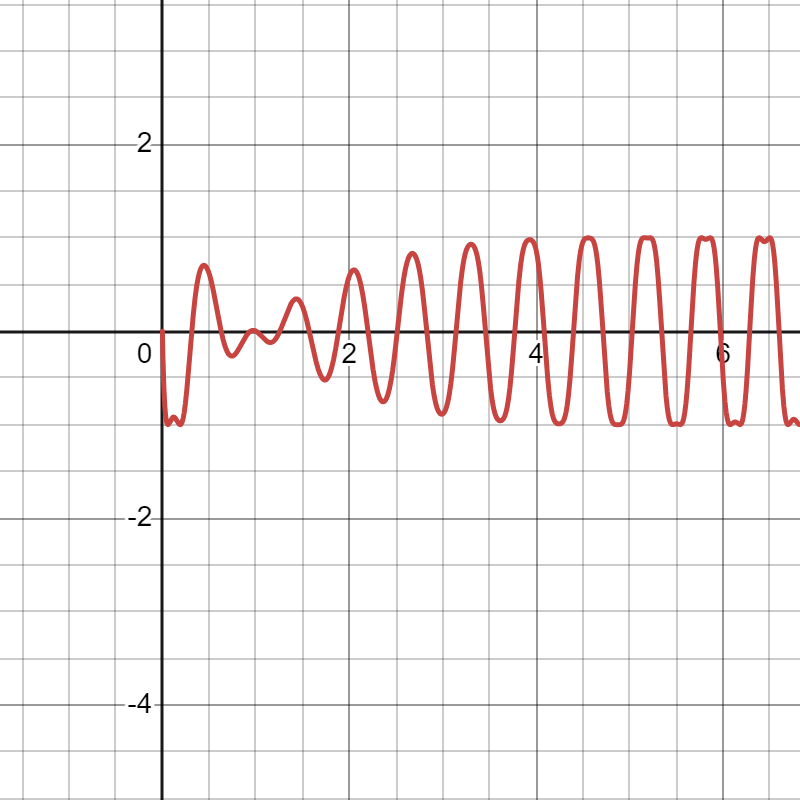
\includegraphics[width=0.5\textwidth]{figures/graph_hardsin.png}
    \caption{График функции $f(x) = \sin\left(\ln(x^{\sin(10x)})\right)$}
    \label{fig:hardsin_graph}
\end{figure}

\subsubsection{Добавление шума}

Для повышения устойчивости модели и её способности к обобщению в процессе обучения на тренировочные данные добавлялся шум, который следовал нормальному распределению. Это позволяет модели лучше адаптироваться к реальным данным, которые часто содержат случайные колебания и погрешности. Нормальное распределение (также называемое гауссовским распределением) является одним из наиболее часто используемых видов распределений в статистике и машинном обучении.

\paragraph{Формула нормального распределения:}
Нормальное распределение определяется следующей плотностью вероятности:

\[
f(x) = \frac{1}{\sqrt{2 \pi \sigma^2}} e^{-\frac{(x - \mu)^2}{2 \sigma^2}}
\]

где:
\begin{itemize}
    \item $\mu$ - математическое ожидание (среднее значение),
    \item $\sigma$ - стандартное отклонение (мера разброса данных),
    \item $x$ - случайная величина.
\end{itemize}

Параметры $\mu$ и $\sigma$ в нашем случае были рассчитаны на основе целевой переменной тренировочного датасета $\texttt{train\_data\_y}$, чтобы шум соответствовал масштабу данных.

\paragraph{Применение шума в датасете:}
Добавление шума выполнялось с использованием библиотеки NumPy, где функция \texttt{np.random.normal()} генерирует массив случайных значений, следующих нормальному распределению. В нашем случае среднее значение шума $\mu = 0$, а стандартное отклонение рассчитывается как $0.1 \cdot \sigma$, где $\sigma$ --- стандартное отклонение значений целевой переменной. Формула добавления шума выглядит следующим образом:

\[
\texttt{train\_data\_y\_noisy} = \texttt{train\_data\_y} + \xi, \quad \xi \sim \mathcal{N}(0, 0.1 \cdot \sigma)
\]

\subsubsection{Загрузка и обработка данных}
Для создания тренировочного и валидационного наборов данных использовались встроенные методы генерации датасетов в \texttt{DEGANN}, которые позволяют сохранять данные в формате \texttt{.csv} для последующего использования.


\subsubsection{Временные последовательности}
Рекуррентные нейронные сети, такие как GRU, предназначены для обработки временных последовательностей. Их ключевая особенность заключается в возможности сохранять информацию о предыдущих состояниях для анализа текущих данных. Это делает их идеальными для задач, где данные зависят от контекста, например, аппроксимация временных рядов.

Для корректной работы RNN данные из исходного датасета были преобразованы в последовательности фиксированной длины с помощью функции \texttt{create sequences}:

\begin{lstlisting}[language=Python, breaklines, caption=Создание временных последовательностей,numbers=left]
def create_sequences(data_x, data_y, time_steps):
    x, y = [], []
    for i in range(len(data_x) - time_steps):
        x.append(data_x[i:i + time_steps])
        y.append(data_y[i + time_steps])
    return np.array(x), np.array(y)

time_steps = 10
train_data_x, train_data_y = create_sequences(train_data_x, train_data_y, time_steps)
val_data_x, val_data_y = create_sequences(val_data_x, val_data_y, time_steps)
\end{lstlisting}

В данном примере \texttt{time\_steps} задаёт количество шагов в последовательности. Это означает, что каждый входной элемент сети состоит из \texttt{time\_steps} предыдущих значений, а целевая переменная соответствует следующему значению функции.

\paragraph{Почему RNN работают с временными последовательностями?}
Основное преимущество RNN заключается в их способности передавать информацию через скрытые состояния (\textit{hidden states}). В отличие от обычных нейронных сетей, которые обрабатывают каждый вход независимо, RNN сохраняют информацию из предыдущих шагов и используют её для обработки текущего ввода. Это реализуется через рекуррентную связь, которая обновляет скрытое состояние на каждом временном шаге.



\subsection{Метрики и настройка гиперпараметров}
\label{subsec:metrics}

Для эффективного обучения моделей на основе архитектуры GRU важен тщательный выбор функции потерь, оптимизатора и гиперпараметров. Этот процесс позволяет достичь баланса между качеством аппрокисмации и вычислительными затратами.

\subsubsection{Функция потерь}

В качестве функции потерь использовалась среднеквадратичная ошибка (\textit{Mean Squared Error}, MSE), определяемая формулой:
\[
\text{MSE} = \frac{1}{n} \sum_{i=1}^{n} (y_i - \hat{y}_i)^2,
\]
где \( y_i \) — истинное значение, \( \hat{y}_i \) — предсказание модели, \( n \) — количество примеров.

Среднеквадратичная ошибка была выбрана по следующим причинам:
\begin{itemize}
    \item MSE минимизирует крупные отклонения между истинными и предсказанными значениями, что особенно полезно при аппроксимации сложных функций.
    \item Эта метрика стандартна для задач регрессии и обеспечивает устойчивую сходимость моделей \cite{Goodfellow}.
\end{itemize}

Таким образом, MSE является подходящим выбором для задач, связанных с аппроксимацией решений дифференциальных уравнений.

\subsubsection{Гиперпараметры модели}

Для данной архитектуры были выбраны параметры, исходя из результатов экспериментов и тестов, при которых наблюдался хороший результат при доступном времени обучения и количестве эпох. Проведённые эксперименты позволили определить следующие параметры:
\begin{itemize}
    \item \textbf{Количество слоёв}: 5;
    \item \textbf{Количество нейронов в каждом слое}: 30.
\end{itemize}

Выбор таких параметров обусловлен следующими факторами:
\begin{itemize}
    \item Увеличение числа слоёв и нейронов значительно повышает сложность модели и требуют большего времени обучения. При этом избыточное увеличение параметров не всегда приводит к заметному улучшению качества, а ограниченные ресурсы накладывают свои ограничения.
    \item Уменьшение количества слоёв или нейронов приводит к недообучению модели, что негативно сказывается на качестве аппроксимации функций.
    \item В выбранной конфигурации модель способна эффективно решать задачи аппроксимации, оставаясь достаточно компактной.
\end{itemize}

\subsubsection{Оптимизатор}

Для оптимизации был выбран \textit{Adam}, поскольку он эффективно регулирует скорость обучения для каждого параметра и демонстрирует высокую стабильность в задачах регрессии \cite{HOML}. \textit{Adam} сочетает преимущества методов \textit{Momentum} и \textit{RMSprop}, что делает его особенно полезным при обучении рекуррентных сетей, таких как GRU.

Преимущества выбора оптимизатора \textit{Adam}:
\begin{itemize}
    \item Автоматическая адаптация шага обучения для быстрого достижения сходимости.
    \item Хорошие результаты при обучении моделей, работающих с временными последовательностями \cite{adam}.
    \item Стабильность градиентного спуска, что особенно важно для задач с длительными зависимостями.
\end{itemize}

Таким образом, выбор MSE в качестве функции потерь, использование оптимизатора \textit{Adam} и разумная конфигурация гиперпараметров обеспечивают эффективное обучение модели. Данная настройка параметров позволяет достичь приемлемого качества аппроксимации функций в условиях ограниченных вычислительных ресурсов.

% !TeX spellcheck = ru_RU
% !TEX root = vkr.tex

\section{Эксперимент}
Цель экмперемента - обучить и сравнить модели с полносвязной и рекуррентной архитектурами с одинаковым количеством слоев и нейронов в качестве аппроксимации встроенных в DEGANN функций, а так же на реализованной сложно-аппроксимируемой функции. Сравнить время обучения, показания лосс функций, а так же качество аппроксимации.

\subsection{Условия эксперимента}
\begin{itemize}
    \item Количество слоев: 5
    \item Количество нейронов в каждом слое: 30
    \item Количество эпох (несколько тестов):
    \begin{itemize}
        \item 100
        \item 200
        \item 500
        \item 1000
    \end{itemize}
\end{itemize}
%\subsection{Используемое железо}
%\begin{itemize}
%    \item Процессор: Intel i5 1240p
%    \item Видеочип: Iris Xe Graphics G7 80EUs
%    \item ОЗУ: 16 гб
%\end{itemize}

\subsection{Исследовательские вопросы}
\begin{description}
    \item[RQ1]: Лучше ли реккурентная сеть справляется с аппроксимацией уравнений, встроенных в DEGANN?
    \item[RQ2]: Насколько существенна разница в аппроксимации реккурентной сети и полносвязной?
\end{description}

\subsection{Итоги}
На данном этапе работы, внедренная архитектура находится на этапе тестирования. Эксперемент еще не до конца завершен и его содержание еще не до конца написано.

%\subsection{Метрики}
%%
%%Как мы сравниваем, что результаты двух подходов лучше или хуже:
%%\begin{itemize}
%%    \item Производительность.
%%    \item Строчки кода.
%%    \item Как часто алгоритм \enquote{угадывает} правильную класси\-фикацию входа.
%%\end{itemize}
%%
%%\noindent Иногда метрики вырожденные (да/нет), это не очень хорошо, но если в области исследований так принято, то ладно.
%%Если метрики хитрые (даже IoU или $F_1$-меру можно считать хитрыми), разберите их в обзоре, пояснив, почему выбраны именно такие метрики.
%
%\subsection{Результаты}
%
%%Результаты понятно что такое.
%%Тут всякие таблицы и графики, как в таблице \ref{time_cmp_obj_func}.
%%Обратите внимание, как цифры выровнены по правому краю, названия по центру, а разделители $\times$ и $\pm$ друг под другом.
%%
%%Перед написанием данного раздела имеет смысл проконсультироваться с литературой по проведению экспериментов~\cite{SmirnovCheatsheet}.
%%
%%Скорее всего Ваши измерения будут удовлетворять нормальному распределению, в идеале это надо проверять с помощью критерия Кол\-могорова и т.п.
%%Если критерий этого не подтверждает, то у Вас что-то сильно не так с измерениями, надо проверять кэши процессора, отключать Интернет во время измерений, подкручивать среду исполне\-ния (англ. runtime), что\-бы сборка мусора не вмешивалась и т.п.
%%Если критерий удовлетворён, то необходимо либо указать мат. ожидание и доверительный/предсказы\-вающий интервал, либо мат. ожидание и среднеквадратичное отклонение, либо, если совсем лень заморачиваться, написать, что все измерения проводились с погрешностью, например, в 5\%.
%%Не приводите слишком много значащих цифр (например, время работы в 239.1 секунды при среднеквадратичном отклонении в 50 секунд выглядит глупо, даже если ваш любимый бенчмарк так посчитал).
%%
%%Замечание: если у вас получится улуч\-шение производительности в пределах погреш\-ности, то это обязательно вызовет вопросы.
%%Если погрешность получилась значительной (больше 10-15\% от среднего), это тоже вызовет вопросы, на которые надо ответить, либо разобравшись, что не так (первый подозреваемый~--- мультимодальное распределение), либо более глубоко статистически проанализировав результаты (например, привести гистограммы).
%%
%%В этом разделе надо также явно ответить на Research Questions или как-то их прокомментировать.
%
%\subsubsection{RQ1} Пояснения
%\subsubsection{RQ2} Пояснения
%
%\subsection{Обсуждение результатов}
%
%%Чуть более неформальное обсуждение, то, что сделано.
%%Например, почему метод работает лучше остальных?
%%Или, что делать со случаями, когда метод классифицирует вход некорректно.
%
%
%\subsection{Воспроизводимость эксперимента}
%
%Это настолько важно, что заслуживает тут своего подраздела (в самой работе не надо, это должно естественно вытекать из разделов выше)~--- эксперимент должно быть можно повторить и получить примерно такие же результаты, как у Вас.
%Поэтому выложите свой код, которым мерили.
%Выложите данные, на которых мерили.
%Или напишите, где эти данные взять.
%Напишите, как конкретно запустить, в каком окружении, что надо дополнительно поставить и т.п.
%Чтобы любой второкурсник мог выполнить все пункты и получить тот же график/таблицу, что у Вас.
%Не обязательно это делать прямо в тексте, можете в README своего репозитория, но где-то надо.

% !TeX spellcheck = ru_RU
% !TEX root = vkr.tex

\section*{Заключение}

В рамках данной работы выполнены следующие задачи:
\begin{itemize}
    \item Разработан и реализован модуль с топологией рекуррентной сети для архитектуры GRU.
    \item Создана модель с архитектурой GRU и интегрированы callback-функции для оптимизации процесса обучения, включая раннее прекращение, сохранение лучшей модели и визуализацию результатов.
    \item Подготовлен специальные датасеты для тестирования, а так же добавлена сложно-аппроксимируемая функция \texttt{hardsin}, реализовано добавление шума в датасет для повышения устойчивости модели.
    \item Проведён подбор метрики (MSE) и настройка гиперпараметров, обеспечивающая хорошие результаты и баланс между качеством аппроксимации и вычислительными затратами.
\end{itemize}

Работа на данном этапе продемонстрировала успешную интеграцию архитектуры GRU в пакет DEGANN.

\textbf{Планы на продолжение работы}


Для дальнейшего расширения функциональности системы планируется:
\begin{itemize}
    \item Разработать собственную (кастомную) реализацию слоёв GRU для расширения функциональности настройки сети.
    \item Завершить тестирование архитектуры на различных наборах данных и провести более глубокий анализ результатов, представив их в итоговом эксперименте.
\end{itemize}

\textbf{Код и результаты}


Код, написанный в ходе работы, свободно доступен здесь: \href{https://github.com/Denigmma/degann/tree/RNN_GRU}{https://github.com/Denigmma/degann/tree/RNN_GRU}



\setmonofont{CMU Typewriter Text}
\bibliographystyle{ugost2008ls}
\bibliography{vkr}

\end{document}
